%%%%%%%%%%%%%%%%%%%%%%%%%%%%%%%%%%%%%%%%%%%%%%%%%%%%%%%%%%%%%%%%%%%%%%%%%%%%%%%%
% Template for USENIX papers.
%
% History:
%
% - TEMPLATE for Usenix papers, specifically to meet requirements of
%   USENIX '05. originally a template for producing IEEE-format
%   articles using LaTeX. written by Matthew Ward, CS Department,
%   Worcester Polytechnic Institute. adapted by David Beazley for his
%   excellent SWIG paper in Proceedings, Tcl 96. turned into a
%   smartass generic template by De Clarke, with thanks to both the
%   above pioneers. Use at your own risk. Complaints to /dev/null.
%   Make it two column with no page numbering, default is 10 point.
%
% - Munged by Fred Douglis <douglis@research.att.com> 10/97 to
%   separate the .sty file from the LaTeX source template, so that
%   people can more easily include the .sty file into an existing
%   document. Also changed to more closely follow the style guidelines
%   as represented by the Word sample file.
%
% - Note that since 2010, USENIX does not require endnotes. If you
%   want foot of page notes, don't include the endnotes package in the
%   usepackage command, below.
% - This version uses the latex2e styles, not the very ancient 2.09
%   stuff.
%
% - Updated July 2018: Text block size changed from 6.5" to 7"
%
% - Updated Dec 2018 for ATC'19:
%
%   * Revised text to pass HotCRP's auto-formatting check, with
%     hotcrp.settings.submission_form.body_font_size=10pt, and
%     hotcrp.settings.submission_form.line_height=12pt
%
%   * Switched from \endnote-s to \footnote-s to match Usenix's policy.
%
%   * \section* => \begin{abstract} ... \end{abstract}
%
%   * Make template self-contained in terms of bibtex entires, to allow
%     this file to be compiled. (And changing refs style to 'plain'.)
%
%   * Make template self-contained in terms of figures, to
%     allow this file to be compiled. 
%
%   * Added packages for hyperref, embedding fonts, and improving
%     appearance.
%   
%   * Removed outdated text.
%
%%%%%%%%%%%%%%%%%%%%%%%%%%%%%%%%%%%%%%%%%%%%%%%%%%%%%%%%%%%%%%%%%%%%%%%%%%%%%%%%

\documentclass[letterpaper,twocolumn,10pt]{article}
\usepackage{usenix2019_v3}

% to be able to draw some self-contained figs
\usepackage{tikz}
\usepackage{amsmath}
\usepackage{cite}
\usepackage{tabularx}
\usepackage{indentfirst}
\setlength{\parindent}{1em}
\usepackage{graphicx}
\usepackage{subcaption}
\usepackage{caption}


% inlined bib file
\usepackage{filecontents}


%-------------------------------------------------------------------------------
\begin{document}
%-------------------------------------------------------------------------------

%don't want date printed
\date{}

% make title bold and 14 pt font (Latex default is non-bold, 16 pt)
\title{\Large \bf Minimizing Compaction Impact via Unified Data Format for LSM}

%for single author (just remove % characters)
\author{
	{\rm  Jinghuan YU, Xuan Sun, Chun Jason Xue, Cheng Ji}\\
	Department of Computer Science, City University of Hong Kong\\
} % end author
\maketitle

%-------------------------------------------------------------------------------
\begin{abstract}
%-------------------------------------------------------------------------------
Combining NVM (non-volatile memory) with LSM(log-structured-merged tree) has received extensive attention recently, researchers are interested in how can these byte-addressing materials help to improve LSM's weaknesses. Recent solutions mostly focus on how to access faster for one part of the LSM's components while we evaluate there are still gaps between different storage components. Inspired by the evaluation upon conversion costs for SST (Sorted String Table) files to different memory processable data block formats, we design a unified data format for JigsawDB to achieve light overhead data conversion. We describe the prototype of JigsawDB, a single storage LSM-based system, which can reduce the overhead of data conversion among different storage systems by unified data blocks. This united format produces much less overhead than traditional transformation process. At last, we evaluate the JigsawDB's performance against LevelDB and its hierarchical architecture equipped with NVM. As a result, JigsawDB accelerates 28.1\% for overall execution in the hybrid storage system while hierarchical solution only improves 17.19\%.
\end{abstract}


%-------------------------------------------------------------------------------
\section{Introduction}
%-------------------------------------------------------------------------------

LSM Tree is a high warm writing performance data structure proposed in 1996\cite{o1996log}, gets widely used in many products like  Cassandra\cite{ApacheCa22:online}, Hbase\cite{ApacheHB26:online}, BigTable\cite{chang2008bigtable} and WiredTiger\cite{WiredTig38:online}. LSM uses incremental changes to optimize write throughput, converts random write operations into sequential accessing. However, this introduces extra overheads in space cost and garbage collection. Moreover, when system's persistent component (the stored files) grows larger and larger, the query performance becomes relatively low, repeated records have not been updated in-time will remain in files will lead to further waste of storage space. The additional collection operations (also known as Compaction) applied to these data will introduce further space amplification. Many studies have been researched to improve this problem\cite{dayan2017monkey,dayan2018dostoevsky,kaiyrakhmet2019slm,kannan2018redesigning,raju2017pebblesdb,wu2015lsm,sears2012blsm} since many years ago.

NVM (non-volatile memory) represents the storage materials with byte-addressability, persistent and high random access throughput. These materials such as PCM (phase change memory), MRAM (Magnetoresistive RAM) can provide fast random access on persistent data, improving throughout and reduce failure-recovery. Novelsm\cite{kannan2018redesigning} and SlM-DB\cite{kaiyrakhmet2019slm} provided some successful solutions to improve throughput and control the space amplification, there is still more space to explore.

In this work, we first evaluate the ratio of time spent on different processes during compaction. To our surprise, nearly $\frac{1}{4}$ of time was spent on converting data from file blocks to memory processable format, which is several times larger than the time spent on reading data blocks. To save the overhead of data serialization and de-serialization, this work proposes JigsawDB, a novel design that provides a united format which fits in all storage system. JigsawDB tends to solve the following problems prior proposals haven't finished: (1) \textbf{The conversion costs}: the conversion gap between stored files and in-memory data structures can be eliminated further to optimize the throughput for both read and write operations. (2) \textbf{The wear out problem}: NVM material still suffers the wear out problems, though 3d x-point materials durability is much better than NAND flash devices, directly applying random and piecemeal operations upon NVM is not that wise. (3) \textbf{To ease the impact of compaction}: in-place updates can reduce the frequency of compaction, but it is hard to accelerate this process, by redesigning the data structure on NVM, these new materials can benefit more than just use their performance advantages.

In addition to this, the benefits of organizing data in a more solid format can achieve better compression rate due to the values are logical continuous in real cases. We implement a prototype and evaluate it within an environment equipping a DRAM-emulating NVM and gain 20\% speed up. We are trying to improve the system further to ease the write pause problem brought by Compaction.


\section{Background}
This section provides the background of NVM materials and traditional designs of LSM, introduces the basic features and usage of them, and analyzes the opportunities and challenges while combing these techniques by reviewing several prior works.

\subsection{Non-Volatile Memory}
NVM, or PM (persistent memory), SCM (storage class memory), is the same meaning, referring to a series of memory materials with non-volatile and byte-wise access characteristics. NVM has become a hot topic in recent years, and related research is moving forward. There are many different types of materials like PCM (phase change memory), MRAM (Magnetoresistive RAM), etc. Besides the most noticeable feature, NVM has higher throughput and storage density than traditional NAND flash devices, with the shortages like asymmetrical read/write performance, and limited lifetime leads to the wear-out problems.


Although there is no conclusion on how to use this material, research proposed several main solutions for using this material: 

1. Use NVM as Persistent Transnational Memory, use methods like Redo Logging, Undo Logging, and Log-Structured to manage the transaction and data involved. 

2. Use NVM as a disk to provide better random access performance on blocks and files. For example, introducing the Direct Access (DAX) in Linux. There are also file systems\cite{dulloor2014system} similar to PMFS, NOVA\cite{xu2016nova}, etc.

3. Combining with RDMA in a distributed scenario. Due to the high performance of NVM, the access characteristics of byte addressing, and the access mode of RDMA, distributed NVM + RDMA becomes a new architecture design.


\subsection{Log-Structured-Merged Tree}\label{LSM-introduction}
LSM is designed to provide better write performance than traditional B+ trees. It has the characteristics of sequential write optimized and periodic garbage collection.

\subsubsection{Sequential Write Optimized} 
LSM's basic idea is converting random writes to sequential writes. Most of the storage devices have the characteristics that can perform much better in sequential operations than in random access operations, no matter read or write. LSM caches the newest changes inside the memory and uses batch processing to write down those cached data. Besides, to aggregate the operations, recently updated data will overwrite in memory and be flash to the file system only for the last version.
\subsubsection{Periodic Garbage Collection} 

For using log-structure and an incremental update strategy to persistent operations, data stored in files may be outdated periodically due to deletions and updates, so the garbage collection process, also known as ``Compaction'', is needed. During this compaction process, LSM-based system will iterate through part of the persistent data, delete the out-dated data and reorganize the data in a partially sorted manner to keep read optimal.

For this \textit{Compaction} process will walk through all key-value pairs stored in the target files, apply to merge sorting to these entries and write back to the files. Though most of the implementations tried to optimize compaction process, there are still very severe performance impact and resource occupying problems during this process. Fig. \ref{fig:disk_usage} shows the disk usage over time. These problems have been studied from many years ago. There are three main directions to solve these problems. 

\begin{figure}
	\centering
	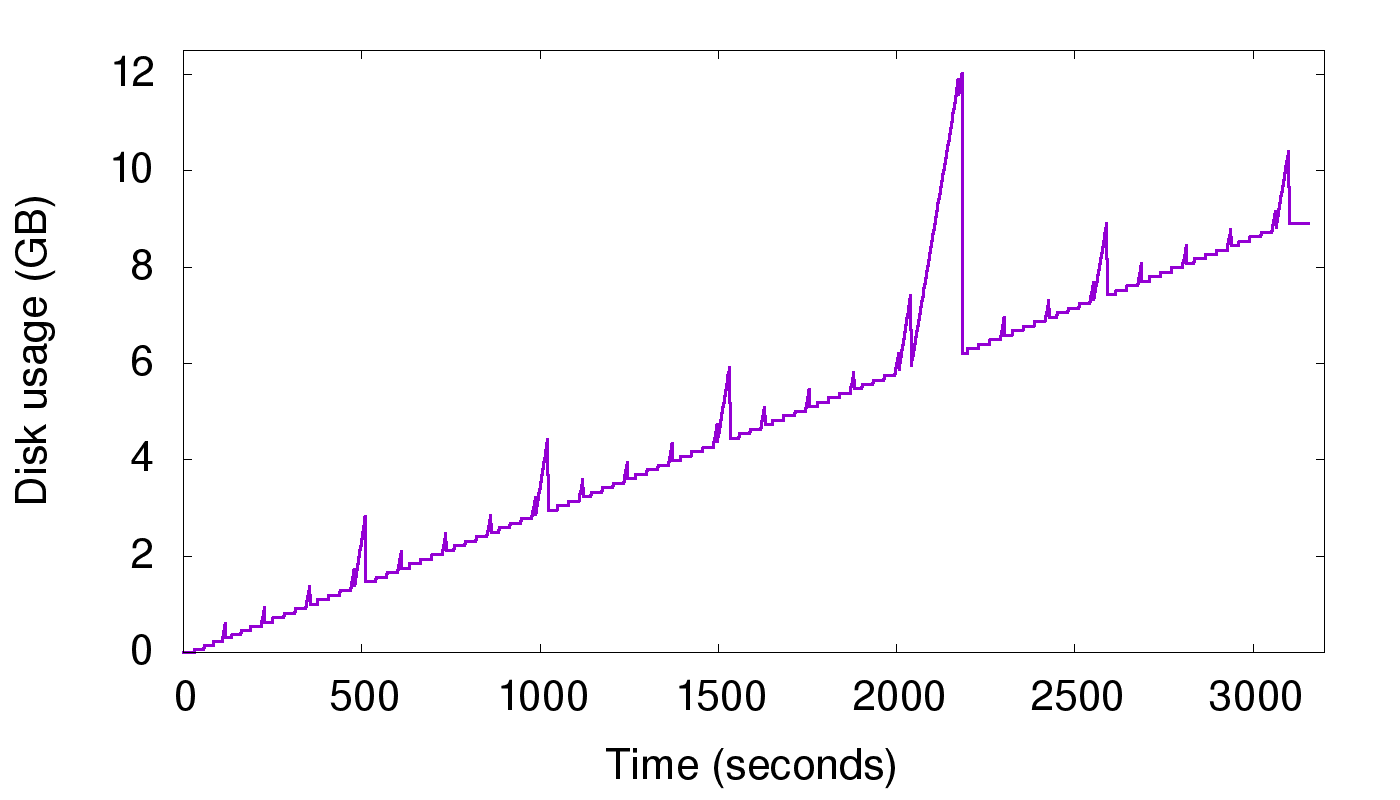
\includegraphics[width=0.9\columnwidth]{fig/compaction-2}
	\caption{The obvious zigzag shape in the disk usage curve, which means the system generate a lot of useless data which is quickly discarded during the compaction process.}
	\label{fig:disk_usage}
\end{figure}

\begin{itemize}
	\item The first one is \textbf{scheduling},  bLSM\cite{sears2012blsm} proposed a ``Gear Scheduler'' to dispersion pressure caused by compaction. It inspired many following works, and most of the work mentioned in this paper used bLSM's results as the baseline while discussing scheduling problems. 
	\item     The second one is \textbf{algorithm optimization}, the most successful and representative one is PebblesDB in 2017\cite{raju2017pebblesdb}, use ``Guard'' to avoid repeated writing entries into files, easing the pressure by reducing write amplification. There are also works focus on specific workloads like LSM-trie\cite{wu2015lsm}. Moreover, this may be the most popular thoughts in practice; Facebook provides several different types of compaction in RocksDB\cite{Compacti60:online},\cite{dong2017optimizing} while Cassandra also changed many times for its compaction strategy\cite{Document20:online}.  
	\item The third one is about \textbf{takeing advantages of new storage materials}, for new materials has been developed lot recent years, how these new materials', like Open-Channel SSD\cite{bjorling2017lightnvm} and NVM, characteristics may benefit the LSM data structure becomes an attractive topic to develop. GearDB\cite{yao2019geardb} considered reorganizing the entries choosing strategy to cover the garbage collection on HM-SMR disks. FlashKV\cite{zhang2017flashkv} use Open-Channel SSDs to optimize the compaction process's write amplification, achieved higher GC-efficiency. Novelsm\cite{kannan2018redesigning} utilized the characteristics of NVM's byte-addressing to achieve in-place update while SLM-DB\cite{kaiyrakhmet2019slm} combined with persistent B-Tree to organize the files into one single level and use \textit{select-merging} to get better performance in compaction.
\end{itemize}

\subsection{Opportunities and Challenges}

Programming for NVM is very different from traditional memory or disk programming. This section describes several main challenges while combing the NVM with the LSM structures.


\paragraph{Space Amplification}
%Fundamentally, this problem is unavoidable for any log-based system as the trade-off for update costs and point looking up costs. Some hardware devices like HM-SMR and Open-channel may provide raw disk control to the applications, make it is possible for an application to cover this problem with the device's garbage collection process\cite{zhang2017flashkv}.

Space amplification problem can be the most common shortage of LSM-based systems, but NVM's high throughput of byte-addressing random operations can solve the problem to some extent. NVM's byte addressing ability allows more flexible data structure and operations; Its large capacity also benefits the buffer to store much more data, caching more operations before writing down to the sequential-based devices. From this point of view, the in-place update strategy can reduce space amplification from the very origin purpose. In addition to eliminating WAL(write-ahead-logging), Novelsm\cite{kannan2018redesigning} applied in-place updates on NVM to reduce repeated writing and SLM-DB use persistent B-Tree to solve this problem.


%\subsection{The Problem of Write Pause}
%Paper bLSM\cite{sears2012blsm} proposed the solution ``Gear Scheduling'' to solve the write pause problem, it also pointed out the origin reason of performance jitters is consuming too much calculating resources to keep the files in ordered manners. 
%
%Fig. \ref{fig:compaction-2}. is the disk usage overtime, it shows another very important reason of \textit{Write Pause}, due to the ``leveled'' compaction strategy of LevelDB, there will be a unavoidable chain reaction triggered by one single compaction which may fill up the entire level

\paragraph{Inherent Weakness of NVM}
Although NVM has many advantages, its inherent weaknesses cause special care in designing the data structure on NVM. Ignoring these issues may not take advantage of NVM's high throughput, and even introduce more unexpected situations or performance degradation.

\textbf{Wear Out Problem:} Though it is much better than traditional NAND flash devices, the limited lifetime of NVM still forces developers to consider wear out issues when designing data structures and underlying system layout\cite{dulloor2014system,van2018managing}. Introducing lifetime consideration means data structures with massively update requirements need additional operations to organize data, brings extra overheads for the system. 

\textbf{Asymmetrical Read/Write Performance:} Another challenge brought by NVM is its asymmetrical Read and Write performance\cite{wu2017early}. Read speed can be two to three orders of magnitude faster than write speed; this feature makes NVM more adaptable to read-intensive tasks, and need optimized batch when dealing with write-intensive tasks.


\textbf{Consistency:}\label{sec:8bytes-law} NVM's non-volatile feature also brings consistency problems. Data structure may result in abnormal state while flush into different storage hierarchy caused by the CPU cache and the out-of-order execution of CPU. The uncertain status of data structures means NVM requires a specified \textit{transaction programming} model\cite{volos2011mnemosyne,dulloor2014system,ren2015thynvm,188438} to ensure the semantics of atomic operations are achieved. Moreover, to provide consistent writing on data blocks larger than limited size (8 bytes in typical situations), logging and C-o-W (Copy on Write) is needed, which means it should consider about the alignments for data structures. Fortunately, persistent B+Tree\cite{188438,oukid2016fptree} was once a popular topic and has been fully developed since many years ago, providing many successful cases for us to reference.
%this results in the extra memory fence and cache flush operations to keep consistency.

\paragraph{Frequent serialization and de-serialization} LSM system achieved buffering data inside memory to provide append-only writing strategy, and many of implementations use \textit{MemTable} as an in-memory buffer and \textit{SST} (Sorted String Table) files to store Key-Value pairs in the file system. 

%Use LevelDB\cite{LevelDBo44:online} as an example, while applying a \textit{Get} operation, LevelDB will find in the memory buffer (\textit{Memtable}) firstly, then access the version control to check which file contains the target key-value pair; After locating the file, it still needs several iterators to transfer the file blocks to memory structure, and decode from preamble compression format to get the real value.
 
\begin{table}[t]
	\centering
	\begin{tabular}{|l|c|c|c|c|c|}
		\hline
		\textbf{Operation} & Read & Write & Encode & Decode  \\ \hline
		\textbf{Ratio (extreme)} & 0.7\% & 6\% & 22\% & 5\%  \\ \hline
		\textbf{Ratio (average)} & 0.1\% & 5\% & 14\% & 3\%  \\ \hline
	\end{tabular}
	\caption{Execution time ratio during compaction process, the second row shows a extreme case among the experiments, and the third rows shows the average value of experiment results. For different components shown in first row, \textbf{Read} means reading file blocks from disks; \textbf{Write} means writing blocks to disks; \textbf{Encode} means transfer key-value entries to the block format, mainly consists of a preamble compression for adjacent keys and variable integer encoding process etc. ; \textbf{Decode} means the process transfer blocks back into iterator's buffer and table cache.}
	\label{tab:file_read_ratio}
\end{table}

Table. \ref{tab:file_read_ratio}. shows the time ratio of different operations, from the result we can see \textbf{\textit{Encoding}} cost the most (almost $\frac{1}{4}$ of entire compaction process). Besides, due to the restart placeholder added by the preamble compression groups, the performance of SST files operations performed on NVM will introduce much more overhead than expect, even worse, offsets the advantages of NVM's high-performance read and write.

\section{Preliminary Proposal}
The challenge is to design an LSM-based system with only one single data structure which can serve both inside the memory space and persistent files. A typical unified format may suffer from low compression rate, high memory usage, and low range query speed problems, to get rid of the serialization/de-serialization overhead, the critical point is to find out a memory structure can also perform well in sequential writing occasions. This section analyzes several design principles and exciting results from observations.

This section introduces the abundant of applying SST files on NVM system, combining with design principles, proposes a highly aggregated, 8-byte aligned and self-indexed format adapted to all storage environments.

\paragraph{Abundant of SST on NVM}
Nearly all of the LSM systems suffer from the same shortage of disk-based DB\cite{sauer2018fineline}: the in-memory-abundant. Encoding/decoding, compression, value-addressing, and memory management make LSM relatively slow to apply the queries. Fig. \ref{fig:sstblock} shows the original format of Value Blocks in LevelDB.

\begin{figure}
	\centering
	\includegraphics[width=0.9\columnwidth]{fig/SSTBlock}
	\caption{Original SST file block, this the format of value blocks, keys inside one same block use preamble compression to reduce space overhead.}
	\label{fig:sstblock}
\end{figure}

Though preamble compressed keys cost less space, the de-serialization overhead is relatively high. Moreover, in a byte-addressing memory system needs an alignment, storing an entry all together is not that efficiency, and the most important is: separated value columns become harder to take advantages of the high compression ratio feature of column-based format.


\paragraph{Memory Component Concern}
Table \ref{tab:memtable_requirment}. shows some design principles of the in-memory data structure and lists out the most popular design to fit each requirement\cite{MemTable29:online} (Alternative list: SkipList, HashSkipList, HashLinkList, Vector). The conclusion of this table points out the SkipList, which is the most popular data structure in typical LSM-based system, may be the best data structure to support in-memory and NVM data buffering. Moreover, Novelsm\cite{kannan2018redesigning} and SLM-DB\cite{kaiyrakhmet2019slm}, these two successful studies have already proved that persistent SkipList can perform well on the NVM material.
\begin{table}
	\centering
	\begin{tabular}{|p{0.5\columnwidth}|p{0.3\columnwidth}|}
		\hline
		\textbf{Index Efficiency} & HashSkipList \\ \hline
		\textbf{Full db Scanning Cost} & SkipList \\ \hline
		\textbf{Memory Overhead} & Vectors \\ \hline
		\textbf{MemTable Flush Efficiency} & SkipList \\ \hline
		\textbf{Concurrent Insert} & SkipList \\ \hline
		\textbf{Use Case University} & SkipList\\ \hline
	\end{tabular}
	\caption{Detailed requirements and most suitable structure for \textit{MemTable} designing}
	\label{tab:memtable_requirment}
\end{table}

\begin{figure}[t]
	\centering
	\includegraphics[width=0.9\columnwidth]{fig/KeySet}
	\caption{KeySet format, the united format works for DRAM, NVM and storage devices. For concurrency concern mentioned in section \ref{sec:8bytes-law}, use 8byte as the basic alignment unit for NVM. The index is a flexible field, can convert among different addressing information for all system.}
	\label{fig:keyset}
\end{figure}

\begin{table*}
	\centering
	\begin{tabular}{|c|c|c|c|c|}
		\hline
		\textbf{Solution Cases} & \begin{tabular}[c]{@{}r@{}}Disk + NVM,\\   JigsawDB\end{tabular} & Disk Only, JigsawDB & Disk + NVM, LevelDB & Disk Only, LevelDB \\ \hline
		\textbf{Writing Time Cost (ns)} & 2543407383 & 3100842276 & 2716987809 & 3245228467 \\ \hline
		\textbf{Encoding Time Cost (ns)} & 2650973177 & 4552173256 & 5341669913 & 6872175477 \\ \hline
		\textbf{Total Time Cost (s)} & 46 & 59 & 53 & 64 \\ \hline
	\end{tabular}
	\caption{Time used for different processing part, this should be the baseline for normalizations in the experiment}
	\label{tab:time}
\end{table*}

\begin{figure}[h]
	\centering
	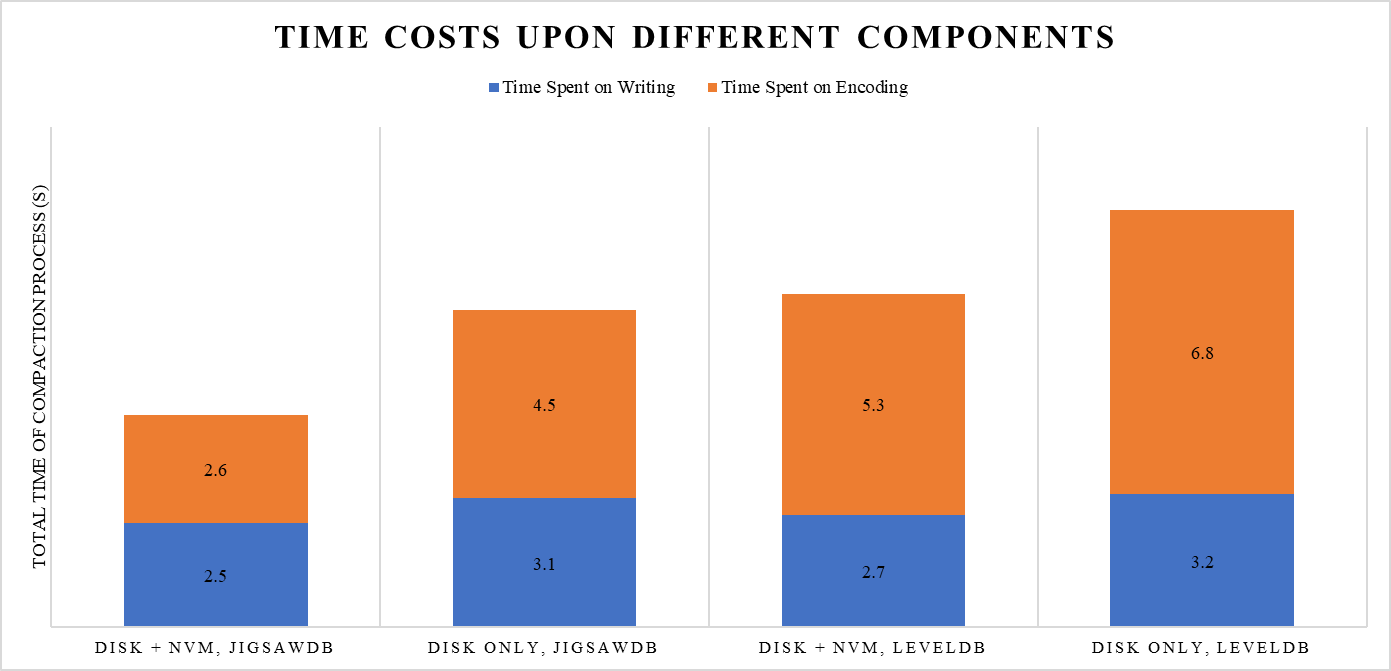
\includegraphics[width=0.7\linewidth]{fig/Time_cost_WE}
	\caption{The absolute value of Writing and Encoding costs}
	\label{fig:timecostwe}
\end{figure}
\begin{figure}[h]
	\centering
	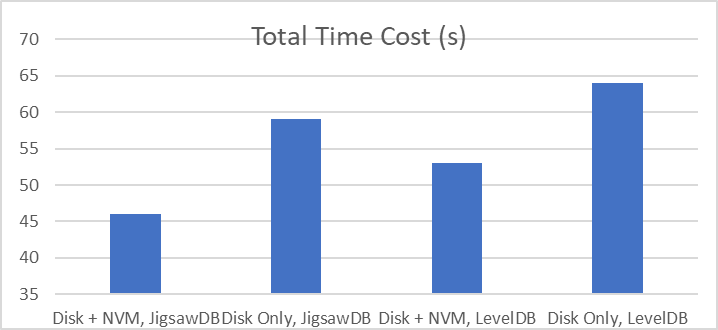
\includegraphics[width=0.7\linewidth]{fig/Time_cost_rest}
	\caption{A more intuitive representation of overall execution time}
	\label{fig:timecostrest}
\end{figure}

\begin{figure*}
	\label{fig:we_values}
	\begin{subfigure}[t]{0.3\linewidth}
		\centering
		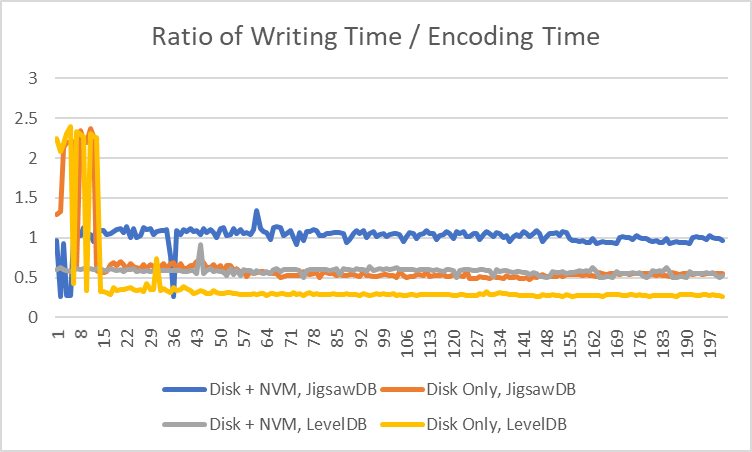
\includegraphics[height= 3cm]{fig/ratio_full}
		\caption{The ratio trend for the whole stage}
		\label{fig:ratiofull}
	\end{subfigure}%
	\hspace{0.5cm}
	\begin{subfigure}[t]{0.3\linewidth}
		\centering
		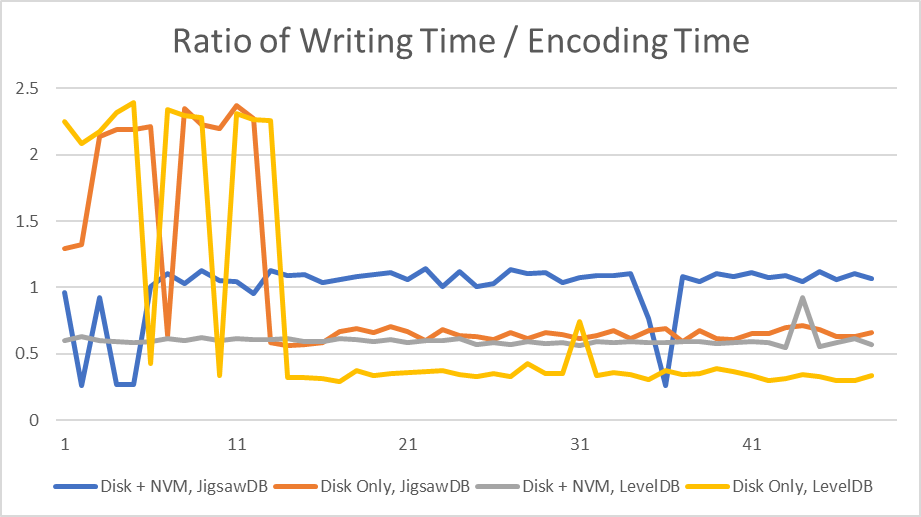
\includegraphics[height= 3cm]{fig/ratio_first_50}
		\caption{The ratio in early stage}
		\label{fig:ratiofirst50}
	\end{subfigure}%
	\hspace{0.5cm}
	\begin{subfigure}[t]{0.3\linewidth}
		\centering
		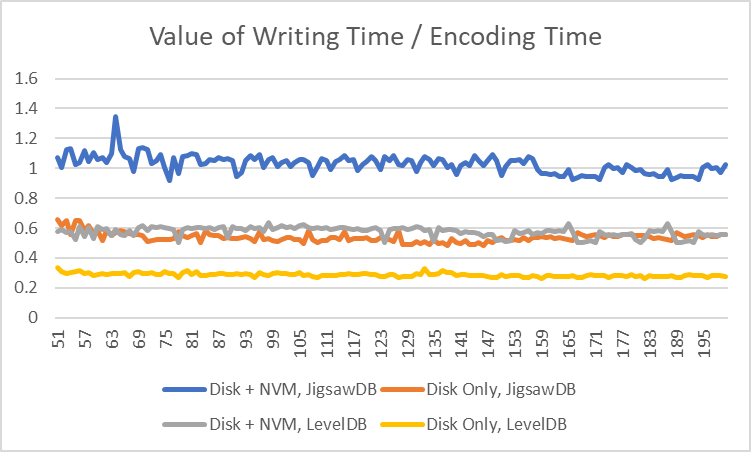
\includegraphics[height= 3cm]{fig/ratio_last_170}
		\caption{The ratio in later stage}
		\label{fig:ratiolast170}
	\end{subfigure}
	\caption{These three figures shows the results of the ratio of Writing Time / Encoding Time. The ordinate in the figures is the specific proportional value while the abscissa represents the process of sampling time.}
\end{figure*}


\paragraph{KeySet Block Files}\label{sec:format_introduction}

Fig. \ref{fig:keyset}. shows the new data structure based on SkipList and SST files. For each block, it contains two components: Key Set and Value Buffer. 
The \textbf{index field} is the crucial point to adapting different storing requirements. This index is a fixed length (8 bytes) filed, which can fit all addressing methods. In the DRAM, it is the pointer of its value slice; when persisted into NVM files, it can be the offset information inside target block; And for the files on disk-based storage, this field will represent a fixed 64 bits value to record an entry'sA value length.

Another component benefits both in NVM, and disk-based storage is the separated value buffer. These data blocks are raw data need no conversion. Though these data can be separated inside DRAM due to dynamic allocation mechanism, the \textbf{Flush} or (\textbf{Memtable Compaction} in another name) can aggregate these data together, become a raw and solid data. In addition, just like the column-based storage engines, gathering value data can gain better compression ratio, for the values are logically continuous.

\section{Evaluation}


\subsection{Workload and Environment Setting}

We use persistent memory workload generated from micro benchmark, perform 100000 operations of the following orders: ``fillseq'', ``fillsync'', ``fillrandom'', ``overwrite'', ``readrandom'', ``readseq'', ``readrandom'', ``readseq'', the key size is 16 bytes and value size is 100 bytes by default. The platform that this experiment performed employs one CPU (8 cores, Intel i7-7700HQ, 2.80GHz) with CPUCache size of 6144 KB. It also contains 24GB DDR4 main memory, and use 8GB of DRAM to emulate the NVM as proposed in former studies\cite{kannan2018redesigning,kaiyrakhmet2019slm}. For the machine, Ubuntu 18.04 LTS with Linux kernel version 4.15 is used.

\subsection{Result Analysis} 
For this is an experiment performed on a prototype, the encoding time we count here includes several data format transfer and value calculation processes rather than preamble compression only. Table. \ref{tab:time}. shows the absolute time cost of file writing, encoding, and the entire process loop. In this experiment, we choose the ratio of writing time as the normalization indicator. For each storage system, the throughput is limited as its inherent property, the higher this value is, the system spends less overhead on conversion.

\paragraph{Data Normalization} The sample data used in Fig. \ref{fig:ratiofull}. is collected among all the compaction information while performing the workload. To observe the results more intuitively, these data points are normalized into 200 equal parts according to the compaction process sequences. 

\paragraph{Numeric Analysis on Time Overhead} From the result in Table. \ref{tab:time}., we can conclude that JigsawDB reduces 28.1\% of the overall execution time compared to the original LevelDB; and is 13.2\% faster than write hierarchically on NVM. As for the effect of this united format, JigsawDB saves 22.03\% of the time while hierarchy methods save only 17.19\% by using NVM. The fact that saving more time by utilizing NVM proves that JigsawDB can benefits more from NVM. At last, due to the fast sequential performance of disks and limited workload size, the benefits of NVM + Disk hybrid architecture does not gain pronounced improvement, this means when data size grows big enough, the performance of JigsawDB can be even better. 

\paragraph{Result Analysis After Normalization} 

From the normalization result, we can find out an interesting fact: for most cases (excepts applying hybrid storage on LevelDB hierarchically) the first quarter of curves (as shown in Fig.  \ref{fig:ratiofirst50}.) fluctuate significantly, but then become stabilized and remain stable for a considerable period of time(as shown in Fig. \ref{fig:ratiolast170}. However, applying hybrid storage structures to LevelDB by extending its memory component can provide much smoother performance. The reason for this behavior is simple, at the early stage of lsm-based system, the size of a single SST file is smaller, which means there are fewer entries stored in one single SST file; in addition, with the entires being aggregated, the keys' value space is becoming dense gradually, and the complexity of finding shared data also growth. 


\section{Discussion and Work-in-progress}
In this paper we introduce the JigsawDB, a novel lsm-based system uses a united format for DRAM, NVM, and disk storage. We implement the prototype of it and evaluate this prototype to validate our design purples to reduce serialization overhead. From the experiment, Jigsaw proves this united format can save the cost of serialization and de-serialization, improve the total performance against original SST files, benefit more among NVM's high throughput read and write features than naively deploy single component upon NVM. But there are still many improvements we can provide.

\paragraph{In-place Update Strategy}
Just as the proposal of Novelsm\cite{kannan2018redesigning} suggests, NVM's byte addressing ability can benefit much in reducing space amplification for cutting off extra overhead of appending record produced in updating. Just as mentioned in section \ref{sec:format_introduction}, entries can be directly addressed inside NVM, and since entries are stored in a compacted, solid data block, the traditional punch-out strategy may leave lots of sporadic memory fragments. We are working on applying a relaxation algorithm to provide in-place update and ensure won't introduce more calculating or serialization overhead.

\paragraph{Control the Write Pause}
Another extreme impact that compaction may bring is \textit{write pause}, which is caused by sudden increment of disk usage, exhausted the bandwidth of the platform. BLSM uses the gear scheduler to reduce the impact of write pause; we are inspired by this to apply a pre-load protocol to take benefits of united format, which can distribute the pressure of the process into the NVM component to reduce the sudden increasing throughput.
%-------------------------------------------------------------------------------
\bibliographystyle{plain}
\bibliography{main}

%%%%%%%%%%%%%%%%%%%%%%%%%%%%%%%%%%%%%%%%%%%%%%%%%%%%%%%%%%%%%%%%%%%%%%%%%%%%%%%%
\end{document}
%%%%%%%%%%%%%%%%%%%%%%%%%%%%%%%%%%%%%%%%%%%%%%%%%%%%%%%%%%%%%%%%%%%%%%%%%%%%%%%%

%%  LocalWords:  endnotes includegraphics fread ptr nobj noindent
%%  LocalWords:  pdflatex acks
